%!TEX root = ..\Gus-thesis.tex
\glsresetall

\chapter{Affine input estimation method}\label{chap:AffineInput}


\begin{quote}
\vspace{-0.5cm}
\emph{The results of this chapter were published in Quintana Carapia, G., and Markovsky, I.,
"Input parameters estimation from time-varying measurements", Measurement Journal, Vol. 153, 2020,
ISSN 0263-2241, doi:10.1016/j.measurement.2019.107418. \nocite{QuintanaMEAS} }\vfill{}
\end{quote}

%\vfill{}

%\section{Introduction}

\color{blue} 
In this thesis document we have discussed that a measurement estimates the unknown value of a physical quantity, also called measurand.
The physical quantity of interest is applied as an input signal to a dynamic system, the sensor, and its state changes from the initial conditions into a transient state.
The input value is estimated using the sensor response in transient state.
A dynamic measurement occurs when the input fluctuations impacts on the input value estimation.
A typical example of a dynamic measurement problem is a low-bandwidth sensor excited with a fast changing input as is explained in \citet{Dienstfrey14}.
In this case, the sensor transient response is slower than the variation of the input, making it difficult to track the input evolution.
The variation of some input characteristics, like the minimum or maximum or the effects of the environment, are considered in applications such as measurements of temperature in \citet{Saggin01}, pressure in \citet{Matthews14}, acceleration in \citet{Link07}, force in \citet{Vlajic16, Hessling08a}, and mass in \cite{Shu93, Boschetti13}.

The data-driven step input estimation method, introduced by \citet{Markovsky15cep} and described in Chapter \ref{chap:Preliminaries},
estimates the unknown step level of an input directly from the sensor step response.
Since most inputs have variations, contrary to the step response that is constant after its application, sets the need for methods for estimating more input models.
One of such input models are affine inputs that vary at a constant rate, and they are found in applications where the measurand activates the sensor gradually. 
An example of gradual activation is the mass measurement of objects in motion, that exists in along conveyor belts.

Current solutions to the weighing in motion are low pass filters that estimate the mass using a saturated ramp as it is proposed by \citet{Tasaki07}, and by \citet{Niedzwiecki16b}, and also time varying filters are developed in \citet{Piskorowski08} and in \citet{Pietrzak14}.
Nevertheless, the signal processing affine input estimation methods are motivated by the need to obtain the mass of the object from the ramp before it reaches saturation.
The ramp is parameterized as a straight line model where the slope and the interception are the parameters of interest of an affine input model.
This chapter describes two methods for the estimation of the affine input parameters.

One method is an extension of the data-driven step input estimation method, and then it is a recursive algorithm of low computational cost that can be implemented in real-time.
The second method is a maximum-likelihood (ML) estimation method based on local-optimization that is proposed for off-line processing of the sensor transient response.
The ML method is similar to the model predictive control approach, as discussed in \cite{Mayne14}, because a cost function is minimized iteratively to optimize the parameters of a sensor model using the observed sensor response in a receding time horizon.
The difference is that the ML method aims to estimate the unknown value of the affine input parameters instead of identifying a model and controlling the dynamic system.
Nevertheless, the ML method can estimate the parameters of the affine input, the parameters of a sensor model, and the initial conditions of the sensor.

The uncertainty of the subspace method is assessed in \cite{QuintanaCSDA} using a Taylor expansion of the estimate and Monte Carlo random sampling approach.
The Monte Carlo approach requires a large set of generated random samples, and according to \citet{Cox06}, for simple systems it is the recommended method.
The uncertainty of the ML method is assessed using the derivatives of the residual error that constructs the to-be-minimized cost function.
The covariance of the optimization method estimate is found in \cite{Pintelon12Book} using the inverse of the Hessian matrix.
\color{black}

\begin{comment}
Measurements estimate the unknown value of a physical quantity, namely the measurand.
The to-be-measured physical quantity is applied as an input signal to a sensor. 
The sensor is a dynamical system and its output changes as a consequence of the input excitation and the sensor initial conditions.
The goal of a measurement is to estimate accurately the measurand value using the sensor transient response.
The transient response of a stable sensor decays to a steady state response.
In steady state, the most accurate estimation of the input true value is simply found using the sensor static gain.
However, the steady state is reached in theory after an infinite period of time and in practice we require fast estimations.
The trade-off between accuracy and speed exists in all measurements.

The measurand can be assumed to be constant or variable during the measurement.
A dynamic measurement is present when the fluctuations of the measurand impact on the input estimation.
A typical example of a dynamic measurement problem is a low-bandwidth sensor excited with a fast changing input.
Some characteristics of the input, like the minimum or maximum or the effects of the environment on the measured quantity, occur in small periods of time.  
The detection of the input characteristics is needed in several scientific and industrial applications such as measurements of temperature \cite{Saggin01}, pressure \cite{Matthews14}, acceleration \cite{Link07}, force \cite{Vlajic16, Hessling08a} and mass \cite{Shu93, Boschetti13}.

The solution to dynamic measurement problems is non-trivial.
An approach is to add a dynamical system to compensate the sensor transient response, inverting the effects of the sensor dynamics.
The purpose of such a compensator is to reduce the transient time.
The sensor dynamics are considered in the design of finite and infinite impulse response compensation digital filters based on deconvolution \cite{Eichstadt10} or synthesized to correct dynamic errors \cite{Hessling08a}. 
The model-based deconvolution design of compensators implies that the measurand true value should be known a-priori for certain applications, such as mass determinations \cite{Boschetti13, Niedzwiecki16b}.
In the literature most of the measurements systems are assumed linear time-invariant, but the compensation digital filters can be linear \cite{Tasaki07},  nonlinear \cite{Shu93} or time-varying \cite{Pietrzak14}.

The digital signal processors enable a different approach where the input estimation can be obtained with algorithms that do not necessarily recreate the dynamics of a system.
One of the authors of this paper proposed a data-driven signal processing method that estimates the measurand true value using subspace techniques \cite{Markovsky15cep, Markovsky15ieee}.
The subspace estimation method bypasses the model identification step to estimate the unknown input directly from the response data.
This method was developed to estimate inputs modeled as step functions of unknown scaling level.
We extended the subspace input estimation method to estimate the parameters of inputs that vary at a constant rate.

The inputs that vary at a constant rate are found in applications where the measurand activates the sensor gradually. 
An example of this activation is the measurement of mass while the to-be-weighted object is transported by a conveyor belt, and the profile of the input is a saturated ramp.
Current solutions to the weighing in motion are low pass filters that estimate the mass using the saturated ramp \cite{Tasaki07, Pietrzak14}.
The signal processing affine input estimation methods are motivated by the need to obtain the mass of the object from the ramp before it reaches saturation.
The ramp is parameterized as a straight line model where the slope and the interception are the parameters of interest.

This paper describes a subspace method for the estimation of the affine input parameters.
This method is a recursive algorithm that can be implemented in real-time since it has low computational cost.
The subspace method is independent of the sensor model and, therefore, it is suitable for a variety of applications.
The dynamic weighing is one of the applications and was chosen as an implementation example.
The effectiveness of the method is evaluated in a simulation study.
The performance of the proposed method is compared to that of a maximum-likelihood (ML) estimation method based on local-optimization and a time-varying compensation filter.
%We found that the subspace method obtains the slope estimate from the sensor transient response using the same assumptions of the data-driven step input estimation method.

The ML method resembles the model predictive control approach in the sense that a cost function is minimized iteratively to optimize the parameters of a sensor model using the observed sensor response in a receding time horizon \cite{Mayne14}.
The difference is that the ML method aims to estimate the unknown value of the affine input parameters instead of identifying a model and controlling the dynamic system.
The ML method is more appropriate for off-line processing of the sensor transient response.
Nevertheless, the ML method can estimate the parameters of the affine input, the parameters of a sensor model, and the initial conditions of the sensor.

The uncertainty of the subspace method is assessed using a Taylor expansion of the estimate and Monte Carlo random sampling approach \cite{Quintana19}.
The Monte Carlo approach requires a large set of generated random samples, and for simple systems it is the recommended method.
There exists a deterministic sampling approach to study the uncertainty propagation of complex systems \cite{Hessling13a, Hessling13b}. 
Deterministic sampling aims to represent the minimal statistical information that is relevant to the uncertainty estimation in a finite set.
The uncertainty of the ML method is assessed using the derivatives of the residual error that constructs the to-be-minimized cost function.
The covariance of the optimization method estimate is found using the inverse of the Hessian matrix \cite{Pintelon12Book}.

\end{comment}


\section{Affine input estimation problem}

The affine input is modeled as a straight line $u(t) = {a} t + {b}$ with parameters the slope $a$ and the intercept $b$.
The affine input estimation problem is formulated as a signal processing problem as follows. 

\paragraph{Problem} 
Given the sequence of measured output observations $\widetilde{\mathbf{y}} = \left( \widetilde{y}(1),\ldots, \widetilde{y}(\color{blue}N\color{black})\right)$, with $\widetilde{y}(t) \in \mathbb{R}$, of a stable linear time-invariant system of order $n$, and static gain ${G}$, generated by an affine input $u(t) = {a} t + {b}$, estimate the parameters of the affine input, \textit{i.e.,} find the values of the parameters $\widehat{a}, \widehat{b} \in {\rm I\!R}$ such that $\widehat{u}(t) = \widehat{a} t + \widehat{b}$ approximates $u$(t).
The measured observations $\widetilde{\mathbf{y}} = {\mathbf{y}} + \bm{\epsilon}$ are exact sensor responses ${\mathbf{y}}$ perturbed by additive noise  $\bm{\epsilon}$ assumed to be independent and normally distributed of zero mean and given variance $\sigma_{\epsilon}^2$.

\paragraph{Motivating example}
Dynamic weighing is an application example where the affine input can be observed.
The weighing of objects in a conveyor belt gives the sensor input an ideal straight line profile when the conveyor belt moves at a constant speed.
The straight line represents the mass coming gradually into the weighing scale sensor in the conveyor belt, and
the mass can be estimated from the slope $a$ of the straight line model. 
The mechanical vibrations of the conveyor belt perturb the input and the sensor response is affected by measurement noise.
Estimating the mass of the object using the sensor response observations is the ultimate goal.

Consider the weighing scale modeled as a second order mass-spring-damper system, such as the one shown in the diagram of Figure \ref{fig:msd_system}.

\begin{figure}[htb!]
\centering

\begin{tikzpicture}[every node/.style={draw,outer sep=0pt,thick}]
\tikzstyle{spring}=[thick,decorate,decoration={zigzag,pre length=0.3cm,post length=0.3cm,segment length=6}]
\tikzstyle{damper}=[thick,decoration={markings,  
  mark connection node=dmp,
  mark=at position 0.5 with 
  {
    \node (dmp) [thick,inner sep=0pt,transform shape,rotate=-90,minimum width=15pt,minimum height=3pt,draw=none] {};
    \draw [thick] ($(dmp.north east)+(2pt,0)$) -- (dmp.south east) -- (dmp.south west) -- ($(dmp.north west)+(2pt,0)$);
    \draw [thick] ($(dmp.north)+(0,-5pt)$) -- ($(dmp.north)+(0,5pt)$);
  }
}, decorate]
\tikzstyle{ground}=[fill,pattern=north east lines,draw=none,minimum width=0.63cm,minimum height=0.3cm]

\node (M) [minimum width=2.5cm,minimum height=0.05cm] {$m$};
\node (Mu) [minimum width=2.5cm,minimum height=0.75cm,yshift=0.57cm] {$u=at+b$};

\node (ground1) at (M.south) [ground,yshift=-1.5cm,xshift=-0.625cm,anchor=north] {};
\draw (ground1.north west) -- (ground1.north east);
\draw [spring] (ground1.north) -- ($(M.south east)!(ground1.north)!(M.south west)$);

\node (groundc) at (M.south) [ground,yshift=-1.5cm,anchor=north] {}; 
\draw (groundc.north west) -- (groundc.north east);

\node (ground2) at (M.south) [ground,yshift=-1.5cm,xshift=0.625cm,anchor=north] {};
\draw (ground2.north west) -- (ground2.north east);
\draw [damper] (ground2.north) -- ($(M.south east)!(ground2.north)!(M.south west)$);

\node[draw=none,fill=none] at (-0.9cm,-1cm) {$k_{\mathrm{s}}$};
\node[draw=none,fill=none] at (0.15cm,-1cm) {$k_{\mathrm{d}}$};
\node[draw=none,fill=none] at (2.0cm,1.0cm) {$y$};
\draw [-latex,thick]  ++(2.2cm,-1cm) -- +(0cm,2.25cm);

\draw [-latex,thick] (M.east) ++(0,0) -- +(1cm,0);
\draw [line width=0.25mm] (2.2cm,-1cm) -- (2.2cm,1cm);
\draw [line width=0.25mm] (2.1cm,-1cm) -- (2.3cm,-1cm);
\draw [line width=0.25mm] (2.1cm,1cm) -- (2.3cm,1cm);
\draw [line width=0.25mm] (2.1cm,-0.5cm) -- (2.3cm,-0.5cm);
\draw [line width=0.25mm] (2.1cm,0.5cm) -- (2.3cm,0.5cm);
\draw [line width=0.25mm] (2.15cm,-0.25cm) -- (2.25cm,-0.25cm);
\draw [line width=0.25mm] (2.15cm,0.25cm) -- (2.25cm,0.25cm);
\draw [line width=0.25mm] (2.15cm,-0.75cm) -- (2.25cm,-0.75cm);
\draw [line width=0.25mm] (2.15cm,0.75cm) -- (2.25cm,0.75cm);
\draw [line width=0.25mm] (2.1cm,0cm) -- (2.3cm,0cm);

\end{tikzpicture}

\caption{\label{fig:msd_system} A second order mass-spring-damper model represents the dynamic weighing system. The dynamics of the system depend on the affine input. The weighing system is time-varying when the applied input changes with respect to time.} 
\end{figure}

The application of an affine input turns the linear time-invariant system into a linear time-varying system, whose
dynamics depends on the input $u(t) = {a} t + {b}$, as it is described by the differential equation:
\begin{equation} \dfrac{d}{dt} \left( \left( {a} t + {b} + m \right) \dfrac{dy}{dt} \right) + k_{\mathrm{d}} \dfrac{dy}{dt} + k_{\mathrm{s}} y = \left( {a} t + {b} + m \right) g \end{equation}
where $m$ is the mass of the scale, $k_{\mathrm{d}}$ is the damping constant, $k_{\mathrm{s}}$ is the elasticity constant, and $g = 9.81$ $\mathrm{m/s}^2$ is the gravitational acceleration. 

The weighing system admits a state-space representation where the states $x_1=y$ and $x_2=\dot{y}$ are the position and the speed of the weighing scale: 
\begin{equation} \dot{\mathbf{x}} = \begin{bmatrix} 0 & 1 \\ \dfrac{-k_{\mathrm{s}}}{{a} t + {b} + m} & \dfrac{-(k_{{d}} + {a})}{{a} t + {b} + m} \end{bmatrix} \mathbf{x} + \begin{bmatrix} 0 \\ g \end{bmatrix}, \quad y = \begin{bmatrix} 1 & 0  \end{bmatrix} \mathbf{x} . \label{eqn:ltvsystem} \end{equation}

In this chapter we use the dynamic weighing example to illustrate the implementation of the affine input estimation methods.


\section{Solution methods}

This section describes the subspace method for solving the affine input estimation problem.
The procedure is motivated by the step input estimation method that is formulated as a structured errors-in-variables (EIV) problem and is solved using recursive least-squares (RLS).
The exponentially weighted recursive least-squares is a generalization of RLS that allows for the extension of the estimation method to reconstruct the affine input.

A maximum-likelihood (ML) method that performs simultaneous system identification and input estimation is described and its results are used as a reference for the subspace method results.

An example of the subspace method is illustrated with a weighing system.
An existing time-varying (TV) compensation filter that was designed for weighing applications is described briefly.
This TV filter is also used to compare the results of the proposed subspace method.


\subsection{Subspace method}
% \linebreak
The errors-in-variables (EIV) minimization problem (\ref{eqn:min_seiv}) is extended to estimate the affine input parameters.
The profile of an affine input excitation can be reconstructed by solving the structured EIV problem  
\begin{equation} \widehat{\bm{\theta}} = \underset{\bm{\theta}}{\mathrm{argmin}} \ \left\Vert \bm{\Omega}^{1/2} \left( \widetilde{\mathbf{y}} - \widetilde{\mathbf{K}} \bm{\theta} \right) \right\Vert^2_2 . \label{eqn:min_ewrls} \end{equation}
where $\widetilde{\mathbf{y}}$ is the observed affine response, $\widetilde{\mathbf{K}}$ is defined in (\ref{eqn:K0plusnoise}), and
the matrix $\bm{\Omega} \in \mathbb{R}^{(\color{blue}N\color{black}-n) \times (\color{blue}N\color{black}-n)}$ is a diagonal matrix of descending powers of the weight factor $\omega \in [0, 1)$, \textit{i.e.},  $\bm{\Omega} = \mathrm{diag}\left(\omega^{\color{blue}N\color{black}-n}, \ldots, \omega^2, \omega^1 \right)$.
The weight factor $\omega$ is a data selection forgetting factor since it enables to apply different weights to the residuals $\widetilde{\mathbf{y}} - \widetilde{\mathbf{K}} \bm{\theta}$.

The exponentially weighted RLS solution to the problem (\ref{eqn:min_ewrls}) is implemented to facilitate the online implementation of the affine input estimation method.
\color{blue}
The exponentially weighted recursive least-squares (RLS) can solve recursively the estimation problem (\ref{eqn:min_seiv}).
In \citet{Kailath00book} the exponentially weighted RLS algorithm is described as follows

\begin{equation} \begin{aligned} \widehat{\bm{\theta}}(k) &= \widehat{\bm{\theta}}(k-1) + \bm{\kappa}_{k} \left( \widetilde{y}(k) - \widetilde{\mathbf{k}}_{k} \widehat{\bm{\theta}}(k-1) \right) , \\  \bm{\kappa}_{k} &= \omega^{-1} \bm{\Psi}(k-1) \widetilde{\mathbf{k}}_{k}^\top / \left( 1 + \omega^{-1} \widetilde{\mathbf{k}}_{k} \bm{\Psi}(k-1) \widetilde{\mathbf{k}}_{k}^\top  \right) \\ \bm{\Psi}(k) &= \omega^{-1} \left( \mathbf{I} - \bm{\kappa}_{k} \widetilde{\mathbf{k}}_{k} \right) \bm{\Psi}(k-1), \label{eqn:RLS} \end{aligned} \end{equation}
for $k = 2n+1, 2n+2, \ldots$, where $\widetilde{\mathbf{k}}_{k}$ represents the row of $\widetilde{\mathbf{K}}$ that corresponds to the $k\mathrm{-th}$ sample, $\bm{\kappa}_{k}$ is a gain scalar, and $\Psi(k)$ is a covariance matrix.
The estimates and the covariance matrix are initialized using the first $n+1$ samples, i.e.,  
\begin{equation} \begin{aligned} \widehat{\bm{\theta}} (2n+1) &= \left( \widetilde{\mathbf{K}}_{n+1}^\top  \bm{\Omega} \widetilde{\mathbf{K}}_{n+1} \right)^{-1} \widetilde{\mathbf{K}}_{n+1}^\top \bm{\Omega}  \widetilde{\mathbf{y}}_{n+1}, \quad \mathrm{and} \\ \Psi(2n+1) &= \left( \widetilde{\mathbf{K}}_{n+1}^\top \bm{\Omega} \widetilde{\mathbf{K}}_{n+1} \right)^{-1} , \end{aligned} \end{equation} 
where $\widetilde{\mathbf{K}}_{n+1}$ is the matrix $\widetilde{\mathbf{K}}$ with the first $n+1$ rows, and $\widetilde{\mathbf{y}}_{n+1}$ is the vector $\widetilde{\mathbf{y}}$ with the first $n+1$ elements\color{black}.
When $\omega=1$, the exponentially weighted RLS solution is identical to that of the RLS.
When $\omega<1$, the older residuals are weighted with lower values than the residuals of recent observations.
In this way, the solution of the minimization problem depends more on newer data, and less on older data. 

In Figure \ref{fig:sensor_response} we can see an example of the affine input $\mathbf{u}$ that excites a weighing sensor, and the generated response $\widetilde{\mathbf{y}}$.
After the transient effects have diminished, the sensor response is a ramp of the same slope as the input, but with a different intercept due to an offset $\omicron$.
The offset $\omicron$ is explained by the parameter $m$ in the sensor representation given in Figure \ref{fig:msd_system}.
This is the mass of the sensor itself, that is added to the mass of the object under measurement.	
From the point of view of the subspace method, the value of $m$ is unknown, and there is no interest in its estimation.

The exponentially weighted RLS solution to the problem (\ref{eqn:min_ewrls}) provides an affine input  estimation $\widehat{\mathbf{u}}$. 
The affine input parameters $a$ and $b$ are estimated, in a second step, by fitting $\widehat{\mathbf{u}}$ to a straight line using linear regression, as follows
\begin{equation} 
  \begin{bmatrix} 1 & 1  \\ \vdots & \vdots \\ \color{blue}N\color{black} & 1 \end{bmatrix} 
  \begin{bmatrix} \widehat{a} \\ \widehat{b}  \end{bmatrix} = 
  \begin{bmatrix} \widehat{u}(1)-\omicron \\ \vdots \\ \widehat{u}(\color{blue}N\color{black})-\omicron \end{bmatrix}, \label{eqn:LS}
\end{equation}
where it is considered the existance of the offset $\omicron$.   

For each new observation $y(t)$, the estimation $\widehat{\mathbf{u}}$ is updated followed by the RLS update of the slope $\widehat{a}$ and the intercept $\widehat{b}$.
The values of the tuning parameters $\omega$ and $\omicron$ can be obtained in the calibration of the method using the response of the sensor.

The calibration procedure consists in the measurement of an object with a reference mass.
During the calibration, $\omega$ and $\omicron$ are tuned by changing their values aiming to reduce the estimation errors of $\widehat{a}$ and $\widehat{b}$.
This reduction of the estimation errors is observed in the convergence of the affine input parameters towards their true values.

\begin{figure}[!htbp]
\centering
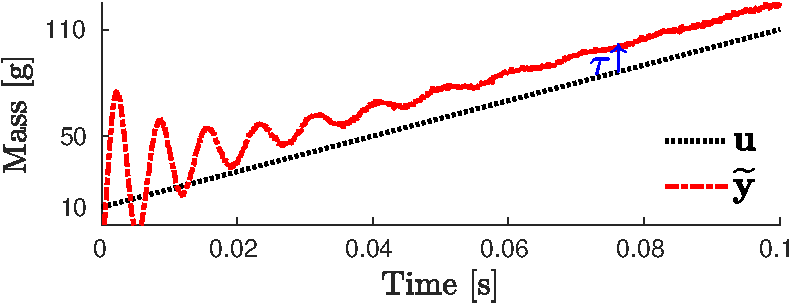
\includegraphics[width=0.69\columnwidth]{./ChapterRampInput/fig/Fig_2_1.pdf} 
\caption{ \label{fig:sensor_response} When the transient part of the sensor response $\widetilde{\mathbf{y}}$ asymptotically decreases, a ramp with the same slope $a$ of the  affine input $u(t) = at+b$ predominates. The intercept of the prevailing ramp is the intercept $b$ added to and offset $\omicron$.}
\end{figure}


The subspace method estimates the input applied to a dynamic system directly from the caused transient response.
This is a recursive method that can be implemented in real time to estimate the input  using low cost digital signal processors.
The method is a model-free approach and can be used in a variety of physical measurements.
The method  tracks any arbitrary time-varying input and can estimate the parameters of the input when it is associated to a particular input model.


\subsubsection{Statistical analysis of the subspace method}

To obtain the first and second moments of the step input estimate $\widehat{\mathbf{u}}$, we need to study the solution
\begin{equation} \widehat{\bm{\theta}} = ( \widetilde{\mathbf{K}}^\top \bm{\Omega} \widetilde{\mathbf{K}}  )^{-1} \widetilde{\mathbf{K}}^\top \bm{\Omega} \widetilde{\mathbf{y}} , \label{eqn:xhatW} \end{equation}
of the overdetermined structured errors-in-variables EIV problem (\ref{eqn:min_ewrls}).
Using a second order Taylor series expansion of the inverse matrix we can approximate the LS solution as
\begin{equation} \widehat{\bm{\theta}} \approx \left( \mathbf{I} - \mathbf{M} + \mathbf{M}^2 \right) \mathbf{C}^{-1} (\mathbf{K} + \mathbf{E})^\top \bm{\Omega} (\mathbf{y} + \bm{\epsilon}). \label{eqn:xhatexpW} \end{equation} 
where 
\begin{equation} \mathbf{C} = \mathbf{K}^\top \bm{\Omega} \mathbf{K}, \quad \text{and} \quad \mathbf{M} = \mathbf{C}^{-1} ( \mathbf{K}^\top \bm{\Omega} \mathbf{E} + \mathbf{E}^\top \bm{\Omega} \mathbf{K} + \mathbf{E}^\top \bm{\Omega} \mathbf{E} ). \end{equation} 

The Taylor series approximation of $\widehat{\bm{\theta}}$ enables the calculation of the estimation bias and covariance since the measurement noise $\bm{\epsilon}$ and $\mathbf{E}$ are no more subject to matrix inversion. 
The bias and the covariance of the estimate $\widehat{\bm{\theta}}$ are obtained from the definitions (\ref{eqn:biasdef}), and (\ref{eqn:covdef}). %The bias and the covariance of the estimate $\widehat{\bm{\theta}}$ are obtained from \begin{equation}  \mathbf{b} \left(\widehat{\bm{\theta}} \right) = \mathbf{\mu} - \widebar{\bm{\theta}}, \label{eqn:biasdef} \end{equation}  \begin{equation} \begin{aligned} \mathrm{\mathbf{Cov}} \left( \widehat{\bm{\theta}} \right) & = \mathbb{E} \left\{ \left( \widehat{\bm{\theta}} - \mathbf{\mu} \right)  \left( \widehat{\bm{\theta}} - \mathbf{\mu} \right)^\top \right\} . \end{aligned} \label{eqn:covdef} \end{equation} where $\mathbf{\mu} = \mathbb{E} \left\{ \widehat{\bm{\theta}} \right\}$ is the expected value of the estimate and $\widebar{\bm{\theta}}$ is the true value. 
Considering the structure of the EIV problem, the bias and the covariance of the estimate approximation (\ref{eqn:xhatexpW}) can be expressed as
\begin{equation} \begin{aligned} \mathbf{b}_{\mathrm{p}} \left( \widehat{\bm{\theta}} \right) & \approx \mathbf{C}^{-1} \left(  \left( \mathbf{K}^\top \bm{\Omega} \mathbf{B}_1 - \mathbf{B}_2 \right) \bm{\theta} - \left( \mathbf{K}^\top \bm{\Omega} \mathbf{B}_3 - \mathbf{B}_4 \right) \right), \end{aligned} \label{eqn:biasEW} \end{equation}
\begin{equation} \begin{aligned} \mathbf{C}_{\mathrm{p}} \left( \widehat{\bm{\theta}} \right) & \approx \mathbf{K}^\dagger \bm{\Omega} \left( \sigma_{\epsilon}^2 \mathbf{I}_{\color{blue}N\color{black}-n} + \mathbf{C}_1 - \mathbf{C}_2 - \mathbf{C}_2^\top \right) \bm{\Omega} \mathbf{K}^{\dagger \top} - \mathbf{b}_{\mathrm{p}} \left( \widehat{\bm{\theta}} \right) \mathbf{b}_{\mathrm{p}}^\top \left( \widehat{\bm{\theta}} \right), \end{aligned} \label{eqn:varEW} \end{equation}
where $\mathbf{B}_1 = \mathbb{E} \Big\{ \mathbf{E} \mathbf{K}^\dagger \bm{\Omega} \mathbf{E} \Big\}$, $\mathbf{B}_2 = \mathbb{E} \Big\{ \mathbf{E}^\top \bm{\Omega} \mathbf{P}_\perp \mathbf{E} \Big\}$, $\mathbf{B}_3 = \mathbb{E} \Big\{ \mathbf{E} \mathbf{K}^\dagger \bm{\Omega} \bm{\epsilon} \Big\}$, $\mathbf{B}_4 = \mathbb{E} \Big\{ \mathbf{E}^\top \bm{\Omega} \mathbf{P}_\perp \bm{\epsilon} \Big\}$, $\mathbf{C}_1 = \mathbb{E} \Big\{ \mathbf{E} \bm{\theta} \bm{\theta}^\top \mathbf{E}^\top \Big\}$, $\mathbf{C}_2 = \mathbb{E} \Big\{ \mathbf{E} \bm{\theta} \bm{\epsilon}^\top \Big\}$, $\mathbf{P}_\perp = \mathbf{I} - \mathbf{K} \mathbf{K}^\dagger \bm{\Omega}$, and $\mathbf{K}^\dagger$ is the pseudo-inverse matrix of $\mathbf{K}$. 

The bias and covariance given by expressions (\ref{eqn:biasEW}) and (\ref{eqn:varEW}) depend on the unobservable true values $\bm{\theta}$ and $\mathbf{K}$.
The measured observations are in the sensor step response $\widetilde{\mathbf{y}}$, and from its observations we construct $\widetilde{\mathbf{K}}$ and compute $\widehat{\bm{\theta}}$.
The substitution of the measured data in the expressions gives an approximation of the estimation bias and covariance. 
We have then
\begin{equation} \begin{aligned} \widetilde{\mathbf{b}}_{\mathrm{p}} \left( \widehat{\bm{\theta}} \right) & \approx \widetilde{\mathbf{C}}^{-1} \left(  \left( \widetilde{\mathbf{K}}^\top \bm{\Omega} \widetilde{\mathbf{B}}_1 - \widetilde{\mathbf{B}}_2 \right) \widehat{\bm{\theta}} - \left( \widetilde{\mathbf{K}}^\top \bm{\Omega} \widetilde{\mathbf{B}}_3 - \widetilde{\mathbf{B}}_4 \right) \right), \end{aligned} \label{eqn:biasSTW} \end{equation}
  \begin{equation} \begin{aligned} \widetilde{\mathbf{C}}_{\mathrm{p}} \left( \widehat{\bm{\theta}} \right) & \approx \widetilde{\mathbf{K}}^\dagger \bm{\Omega} \left( \sigma_{\epsilon}^2 \mathbf{I}_{\color{blue}N\color{black}-n} + \widetilde{\mathbf{C}}_1 - \widetilde{\mathbf{C}}_2 - \widetilde{\mathbf{C}}_2^\top \right) \bm{\Omega} \widetilde{\mathbf{K}}^{\dagger \top} - \widetilde{\mathbf{b}}_{\mathrm{p}} \left( \widehat{\bm{\theta}} \right) \widetilde{\mathbf{b}}_{\mathrm{p}}^\top \left( \widehat{\bm{\theta}} \right), \end{aligned} \label{eqn:varSTW} \end{equation}
  where $\widetilde{\mathbf{B}}_1 = \mathbb{E} \Big\{ \mathbf{E} \widetilde{\mathbf{K}}^\dagger \bm{\Omega} \mathbf{E} \Big\}$, $\widetilde{\mathbf{B}}_2 = \mathbb{E} \Big\{ \mathbf{E}^\top \bm{\Omega} \widetilde{\mathbf{P}}_\perp \mathbf{E} \Big\}$, $\widetilde{\mathbf{B}}_3 = \mathbb{E} \Big\{ \mathbf{E} \widetilde{\mathbf{K}}^\dagger \bm{\Omega} \bm{\epsilon} \Big\}$, $\widetilde{\mathbf{B}}_4 = \mathbb{E} \Big\{ \mathbf{E}^\top \bm{\Omega} \widetilde{\mathbf{P}}_\perp \bm{\epsilon} \Big\}$, $\widetilde{\mathbf{C}}_1 = \mathbb{E} \Big\{ \mathbf{E} \widehat{\bm{\theta}} \widehat{\bm{\theta}}^\top \mathbf{E}^\top \Big\}$, $\widetilde{\mathbf{C}}_2 = \mathbb{E} \Big\{ \mathbf{E} \widehat{\bm{\theta}} \bm{\epsilon}^\top \Big\}$, and $\widetilde{\mathbf{P}}_\perp = \mathbf{I} - \widetilde{\mathbf{K}} \widetilde{\mathbf{K}}^\dagger \bm{\Omega}$. 

The results of the expected values $\mathbf{B}_1$, $\mathbf{B}_2$, $\mathbf{B}_3$, $\mathbf{B}_4$, $\mathbf{C}_1$, and $\mathbf{C}_2$ can be found using Lemma \ref{lem:lemma1}, on page \pageref{lem:lemma1}.
The bias and covariance were obtained to extend the previous analysis conducted on EIV estimation problems without an imposed structure in \citet{Vaccaro94} and \citet{Stewart90SPT}.
It was shown that the bias and variance expressions (\ref{eqn:biasSTW}) and (\ref{eqn:varSTW}) are valid predictions of the first and second moments of the LS estimate of a Hankel structured EIV problem.
The problem formulated by the step input estimation method belongs to this type of structured EIV problems and we can use the derived expressions to find the bias and variance of the input estimate $\widehat{u}$.
The bias of the estimate $\widehat{\mathbf{u}}$ is the fist element of $\widetilde{\mathbf{b}}_{\mathrm{p}} \left( \widehat{\bm{\theta}} \right)$ and the variance of $\widehat{\mathbf{u}}$ is the first element in the main diagonal of $\widetilde{\mathbf{C}}_{\mathrm{p}} \left( \widehat{\bm{\theta}} \right)$.


\subsection{Maximum-likelihood method}

% This means that the ML method implementation depends on the problem under study and not always can be estimated all the sensor model parameters.  
% The identifiability conditions of each sensor model parameter is the requirement to fulfill in order to be estimated with the ML method. %The affine input parameters $a$ and $b$ are the slope and the intercept of the straight line model $u(t) = at + b$.

Using a model of the sensor, the maximum-likelihood ML method simultaneously estimates the parameters of the applied affine input $u(t) = at + b$, and some of the sensor model parameters, \color{blue} using the observed sensor response $\widetilde{\mathbf{y}}$\color{black}.
\color{blue} This method fits iteratively the response of the model $\widehat{\mathbf{y}}(\bm{\theta})$ to the sensor response by searching for the parameters $\bm{\theta}$ that reduce the error difference between both responses.
%the residual $\mathbf{r}(\bm{\theta}) = \widetilde{\mathbf{y}} - \widehat{\mathbf{y}}(\bm{\theta})$ 
Algorithm \ref{Alg1} describes the formulation of an objective function $f = \mathbf{r}^\top \mathbf{r}$, where $\mathbf{r}$ is the residual $\mathbf{r}(\bm{\theta}) = \widetilde{\mathbf{y}} - \widehat{\mathbf{y}}(\bm{\theta})$, that is minimized through the iterations.
The objective function is the sum of the squares of the differences between the samples of both responses.
Since the measurement noise is assumed Gaussian distributed with zero mean and variance $\sigma_{\bm{\epsilon}}^2$, where the samples of this perturbation are independent and identically distributed, the minimization of the objective function $f$ maximizes the likelihood of fitting the actual sensor response with the model response.


The Jacobian matrix of the residual $\mathbf{J}\bm{\theta} = \partial \mathbf{r}(\bm{\theta}) / \partial \bm{\theta}$ can be analytically derived using the sensor model.
With the Jacobian matrix, the ML method searches the direction in which the residual decreases towards a local minimum.
Unfortunately, this ML method cannot guarantee the global minimum since it depends strongly on the initialization of the optimization parameters, as it is discussed in \citet{Nocedal06}.
Therefore, it is proposed to initialize the to-be-optimized parameters $a$ and $b$ using the results of the subspace method obtained after a convenient number of samples so that the affine input parameters are set close to the optimal values.
The initialization of the remaining model parameters under study can be done using the sensor model representation.
An illustrative example of the ML will be provided in a posterior subsection.  
\color{black}

\begin{algorithm} \tag{6.1}
\caption{ML Affine input estimation.}\label{Alg1}
\begin{algorithmic}
  \REQUIRE{$\widetilde{\mathbf{y}}$, and required sensor model parameters}{}
  \STATE {Initialize $\bm{\theta} = (a, b, \text{and \ the \ to-be-estimated \ model \ parameters})$}{}
  \FOR{each $N_{\mathrm{s}}$ observations of $\widetilde{\mathbf{y}}$}{}
  \STATE {Simulate model response $\widehat{\mathbf{y}}(\bm{\theta})$}{}
  \STATE {Obtain residual $\mathbf{r}(\bm{\theta}) = \widetilde{\mathbf{y}} - \widehat{\mathbf{y}}(\bm{\theta})$}{}
  \STATE {Minimize $f = \mathbf{r}^\top \mathbf{r}$ over $\bm{\theta}$}{}
  \STATE {\hspace{0.5cm}  using analytic Jacobian matrix $\mathbf{J}\bm{\theta} = \partial \mathbf{r}(\bm{\theta}) / \partial \bm{\theta}$}{}
  \STATE {Update $\bm{\theta}$}{}
\ENDFOR
\ENSURE {Optimized parameters $\widehat{a}, \ \widehat{b}$, \ and estimated model parameters.} {}

\end{algorithmic}
\end{algorithm}



\subsubsection{Covariance of the ML method estimates}

The ML method simulates a dynamic system, and computes the Jacobian of the residual error in each iteration.
The analytic formulation of the Jacobian benefits the estimation method in two ways: it speeds up the minimization and gives direct access to the variance of the estimates.
The covariance matrix of the ML estimates can be expressed as in \citet{Pintelon12Book}
\begin{equation} \mathbf{C} \left( \widehat{\bm{\theta}} \right) = \sigma_{\bm{\epsilon}}^2 \left( \left( \dfrac{\partial \mathbf{r} }{ \partial \bm{\theta} } \right)^\top \left( \dfrac{\partial \mathbf{r} }{ \partial \bm{\theta} } \right) \right)^{-1}. \label{eqn:covOpt} \end{equation}

The ML estimation method is asymptotically efficient, and the ML estimation variance values are the mininum values that any estimator can attain.
Therefore, the variance of the ML method estimates should be smaller than the CRLB of the structured EIV minimization problem (\ref{eqn:FIM}).

\subsubsection{ML affine input estimation example}

The previously described dynamic weighing system is used to illustrate the ML method implementation.
In this case, the problem can be formulated as: 
 \begin{equation} \begin{aligned}
     & \text{Minimize} \quad \text{over} \ a, b, \mathbf{x}_{\text{ini}} \quad \mathbf{r}^\top \mathbf{r} \text{, subject to:} \\ & \ \dot{\mathbf{x}} = \begin{bmatrix} 0 & 1 \\ \frac{-k_{\mathrm{s}}}{a t + b + m} & \frac{-(a + k_{\mathrm{d}})}{a t + b + m} \end{bmatrix} \mathbf{x} + \begin{bmatrix} 0 \\ g \end{bmatrix}, \\ & \ \widehat{\mathbf{y}} = \begin{bmatrix} 1 & 0  \end{bmatrix} \mathbf{x} .  
 \label{eqn:ltv_abxini} \end{aligned} \end{equation}
where the optimization variables $\bm{\theta} = \left(a, b, \mathbf{x}_{\mathrm{ini}} \right)$ are the affine input parameters $a$, $b$, and the sensor model's initial conditions.

The model parameters $m$, $k_{\mathrm{d}}$, and $k_{\mathrm{s}}$ cannot be estimated simultaneously due to identifiability issues.
In the state equation of the time-varying sensor model, the parameters $k_{\mathrm{d}}$ and $a$ are entangled and cannot be explicitly separated.
The same occurs for the parameters $m$ and $b$, and for $k_{\mathrm{s}}$ with respect to $a$ and $b$.

To define the initial value of the optimization variables $a$, $b$,
the subspace estimation method can be used with, at least, the first $2n+2$ transient response samples, where $n=2$ is the order of the sensor model.
With the initial affine input parameters, a sensor response can be simulated, and, since we are using few samples, the first samples of the simulated response also are an approximation of the initial conditions $\mathbf{x}_{\mathrm{ini}}$.
The optimization variables are updated every $N_{\mathrm{s}}$ new observations.
The minimization algorithm can be, for example, the Levenberg-Marquardt algorithm described in \citet{Nocedal06}. 

The analytic Jacobian matrix $\mathbf{J}$ of the residual $\mathbf{r}(\bm{\theta})$ can be obtained from the first derivative of the state-space representation (\ref{eqn:ltv_abxini}), with respect to the optimization variables $\bm{\theta}$. 
The residual $\mathbf{r}(\bm{\theta}) = \widetilde{\mathbf{y}} - \widehat{\mathbf{y}}(\bm{\theta})$ is the error difference between the observed sensor response $\widetilde{\mathbf{y}}$ and the simulated sensor response $\widehat{\mathbf{y}}(\bm{\theta})$ to the affine input. 
More details of the Jacobian matrix calculation, for the sensor model under study, are given in the appendix.


\subsection{Time-varying compensation filter}

The time-varying (TV) filter described in \citet{Pietrzak14} was designed to compensate the measured responses of a conveyor weighing system, considering they are modeled as a saturated ramp.
The TV filter consists of three low-pass infinite impulse response (IIR) filters in cascade, where the $i-\mathrm{th}$ IIR filter is given by
\begin{equation} \widehat{y}_i(t) + k_1(t) \widehat{y}_i(t-1) = k_2(t) \left( \widehat{y}_{i-1}(t) + \widehat{y}_{i-1}(t-1) \right) \end{equation}
for $i = 1,\ldots,3$ and $t=0, \ldots, \color{blue}N\color{black}$.
The sensor response is fed to the filter, then $\widehat{y}_0(t) = \widetilde{y}(t)$, and the output of the TV filter $\widehat{u}_\mathrm{ltv}(t) = \widehat{y}_3(t)$ is an estimation of the affine input.
Since in our case we are processing only the ramp without the saturation, the estimates $\widehat{a}_\mathrm{ltv}$ and $\widehat{b}_\mathrm{ltv}$ of the input parameters are obtained by fitting a straight line to the estimated input $\widehat{u}_\mathrm{ltv}$ using linear regression.

The time-varying coefficients $k_1(t)$ and $k_2(t)$ are computed in \citet{Pietrzak14} from 
\begin{equation} k_1(t) = \frac{f_c(t) - \frac{k_3}{\pi T_s}}{f_c(t) + \frac{k_3}{\pi T_s}}, \quad k_2(t) = \frac{1 + k_1(t)}{2} , \quad k_3 = \sqrt{ \sqrt[3]{2}  - 1} \end{equation}
where $T_s$ is the sampling time and $f_c(t)$ is a heuristic "cutoff" frequency
\begin{equation} f_c(t) = f_u + \left( f_l - f_u \right) \beta^{\frac{t-1}{\alpha \left( \color{blue}N\color{black}-1 \right)} } \end{equation}
that changes between the lower $f_l$ and upper $f_u$ limits, where the coefficient $\beta$ is lower than one, and $\alpha$ is the decay rate. 
The lower frequency value $f_l$ and the coefficient $\beta$ are fixed and the variables $f_u$ and $\alpha$ are optimized off-line by solving the minimization problem 
\begin{equation} \mathrm{minimize} \ \quad \ \mathrm{over} \ f_u, \alpha \ \quad \ \mathrm{max} \left( \dfrac{\mu_{\widetilde{a}_{\mathrm{ltv}}}}{\mu_{\mathrm{spec}}}, \dfrac{\mu_{\widetilde{b}_{\mathrm{ltv}}}}{\mu_{\mathrm{spec}}}, \dfrac{\sigma_{\widetilde{a}_{\mathrm{ltv}}}}{\sigma_{\mathrm{spec}}}, \dfrac{\sigma_{\widetilde{b}_{\mathrm{ltv}}}}{\sigma_{\mathrm{spec}}} \right) + \mathrm{max} \left( \dfrac{\eta_{i}}{\color{blue}N\color{black}} \right) \label{eqn:tv_optim} \end{equation}
where $\mu_{\widetilde{a}_\mathrm{ltv}}$, $\mu_{\widetilde{b}_\mathrm{ltv}}$, $\sigma_{\widetilde{a}_\mathrm{ltv}}$ and $\sigma_{\widetilde{b}_\mathrm{ltv}}$ are the mean values and the standard deviations of the estimation errors $\widetilde{a}_\mathrm{ltv} = \widehat{a}_\mathrm{ltv} - {a}$, and $\widetilde{a}_\mathrm{ltv} = \widehat{b}_\mathrm{ltv} - {b}$, and where ${a}$ and ${b}$ are the true values of the input parameters.
The values $\mu_{\mathrm{spec}}$ and $\sigma_{\mathrm{spec}}$ are specified in the OIML recommendation R51 defined in \citet{OIML_R51_1} for mass measurements that use a conveyor belt.


\section{Simulation results}
The results of the affine input parameters estimation are discussed in this section.
We performed a simulation study using the weighing system presented as an example.
We compared the performance of the proposed subspace method to a conventional time-varying (TV) filter, that was conceived for weighing applications, and to the maximum-likelihood (ML) method.

A second order weighing system was excited with an affine input to get the transient response.
The parameters of the weighing system are $m$ = 15 g, $k_{\mathrm{d}}$ = 5.5 Ns/m and $kg_{\mathrm{s}}$ = 10250 N/m.
The applied affine input $u(t) = 100 t + 10$ represents a mass that changes from $10$ g to $110$ g, at a constant rate, in a time interval of $0.1$ s.
This change of mass represents one example of the weighing input in a conveyor weighing system when an object of 100 g is measured while it is moving at constant speed.
A total of 1000 samples of the sensor response are acquired with sampling time $T_s = 0.1$ ms.
In Figure \ref{fig:sensor_weight} the input $\mathbf{u}$ is represented with the black dotted line, the red oscillatory curve is the corresponding sensor ramp response $\widetilde{\mathbf{y}}$, and the blue curve $\widehat{\mathbf{u}}_{\mathrm{}}$ is a typic al input estimate obtained with the subspace method.


\begin{figure}[!htbp]
\centering
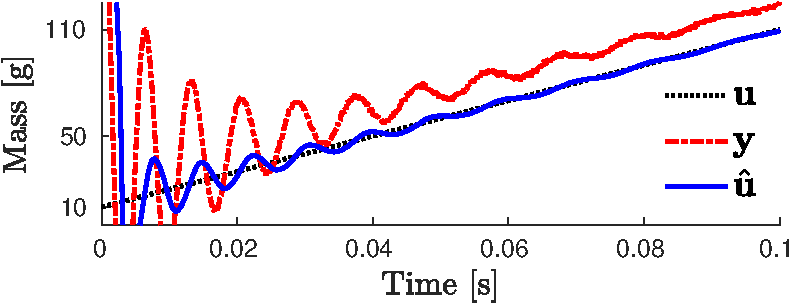
\includegraphics[width=0.69\columnwidth]{./ChapterRampInput/fig/Fig_2.pdf} 
\caption{ \label{fig:sensor_weight} The sensor transient response $\widetilde{\mathbf{y}}$ to an affine input excitation $u(t) = at+b$ is processed by the estimation methods to estimate the parameters $a$ and $b$. In the figure we observe an example of the input estimate $\widehat{\mathbf{u}}$ obtained with the subspace method. The input parameters are calculated from $\widehat{\mathbf{u}} - \omicron$ using linear regression.}
\end{figure}

In each simulation, the sensor response was perturbed with an independent realization of additive normally distributed measurement noise.
The added perturbation noise has signal-to-noise ratio (SNR) in the interval [20 dB, 60 dB].
These SNR values are realistic in practical applications.
The SNR is defined as the ratio of signal power to the noise power, that is equivalent to the root-mean-square (RMS) value of the true signal to the standard deviation of the perturbation noise, and in dB is given by \color{blue}(\ref{eqn:SNR})\color{black}.


\subsection{Results of the subspace method}

The subspace method processed online the sensor transient response.
The first estimation was obtained with $2n+1$ samples, where $n=2$ is the assumed order of the sensor.
The method updated recursively the value of the estimated parameters for each new collected sample, using the forgetting factor $\omega$ listed in Table \ref{table:lambdas}.
In Figure \ref{fig:rele_dd_40dB_s1} we observe the relative errors of the estimates $\widehat{a}$ and $\widehat{b}$ obtained when SNR = 40 dB. 
The relative errors are smaller than 5 \% after 400 and 500 samples are processed, i.e., 0.04 s and 0.05 s, respectively.
As more samples are collected, the parameter estimation improves.
Figure \ref{fig:rele_SNR_dd_10000} shows the final value of the relative errors, found at $t=0.1$ s, for the different SNR values considered.
The relative errors are smaller than 2 \% regardless of the measurement noise level.

\begin{table}[h!]
\centering
\caption{Here are listed the selected values of the forgetting factor $\omega$ and the offset $\omicron$ that configure the subspace method for the different values of SNR. These values were obtained after calibration of the method and were fixed during the simulation study.}
\begin{tabular}{c| c c c c c} 
 \hline
 SNR \ [dB] & 20 & 30 & 40 & 50 & 60 \\ [0.5ex] 
 \hline
 $\omega$ & 0.939 & 0.940 & 0.955 & 0.959 & 0.959 \\ % forgetting factor
 $\omicron$ [g] \  & 15 & 15 & 17 & 14 & 20 \\ [0.5ex] % [\mathrm{samples}]
 \hline
\end{tabular}
\label{table:lambdas}
\end{table}


\begin{figure}[!htbp]
\centering
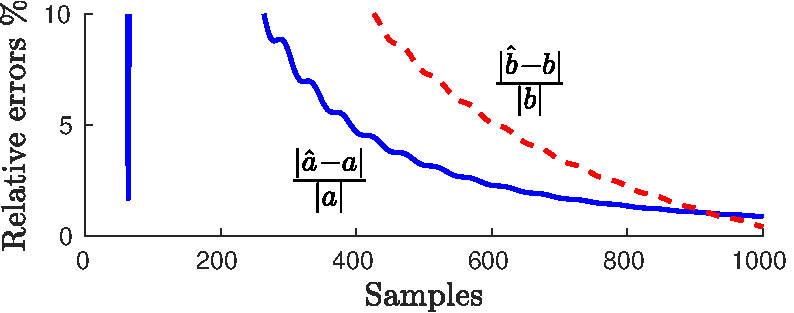
\includegraphics[width=0.69\columnwidth]{./ChapterRampInput/fig/Fig_3.pdf} 
\caption{ \label{fig:rele_dd_40dB_s1} The relative errors of the affine input parameters estimates decrease as the subspace method processes more samples. The relative errors of the estimates $\widehat{a}$ and $\widehat{b}$ are smaller than 5 \% after 400 and 500 samples, respectively ($T_s = 0.1$ ms). }
\end{figure}


\begin{figure}[!htbp]
\centering
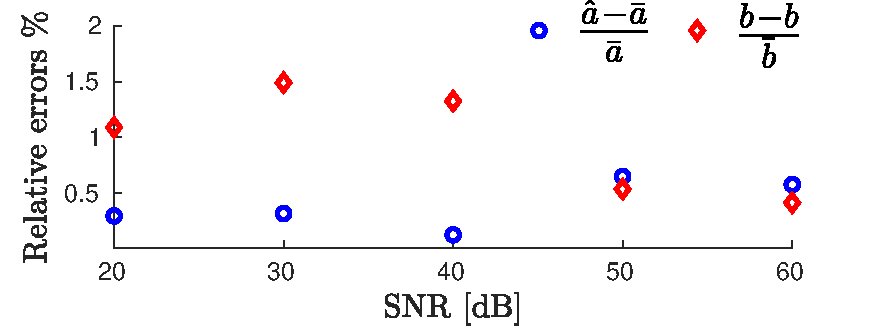
\includegraphics[width=0.69\columnwidth]{./ChapterRampInput/fig/Fig_4.pdf} 
\caption{ \label{fig:rele_SNR_dd_10000} The minimum value of the estimation relative errors obtained with the subspace method is less than 2  \% regardless of the SNR between 20 dB and 60 dB. }
\end{figure}

The Cram\'er-Rao lower bound (CRLB) of the errors-in-variables problem formulated by the subspace method was numerically computed for different sample size using Equation (\ref{eqn:FIM}).
The CRLB is the minimum variance that the estimates $\widehat{a}$ and $\widehat{b}$ can have from the solution of the structured EIV minimization problem. 
The average of $10^4$ runs with independent noise realizations allows to find the empirical mean squared error (MSE) of the estimates, defined as
\begin{equation} \mathrm{MSE}_{\widehat{a}} = \left(b_{\mathrm{p}}\left( \widehat{a} \right) \right)^2 + v_{\mathrm{p}} \left( \widehat{a} \right), \quad \text{and} \quad  \mathrm{MSE}_{\widehat{b}} = ( b_{\mathrm{p}} ( \widehat{b} ) )^2 + v_{\mathrm{p}} ( \widehat{b} ), \end{equation}
where $b_{\mathrm{p}} \left( \widehat{a} \right)$ and $b_{\mathrm{p}} ( \widehat{b} )$ are the bias, and $v_{\mathrm{p}} \left( \widehat{a} \right)$ and $v_{\mathrm{p}} ( \widehat{b} )$ are the variances of the input parameters.
Figure \ref{fig:CRLB_MSE_ab_dd_40dB_MC_10000} shows that the mean squared errors $\mathrm{MSE}_{\hat{a}}$ and $\mathrm{MSE}_{\hat{b}}$ are near to their theoretical minimum $\mathrm{CRLB}_{a}$ and $\mathrm{CRLB}_{b}$ within two orders of magnitude, when SNR = 40 dB.
Figure \ref{fig:CRLB_MSE_SNR_ab_dd_MC_10000} shows the final value of the Cram\'er-Rao lower bounds and the empirical mean-squared errors, found at $t=0.1$ s, for the different SNR values considered.
Both $\mathrm{MSE}_{\hat{a}}$ and $\mathrm{MSE}_{\hat{b}}$ are less than one order of magnitude near to $\mathrm{CRLB}_a$ and $\mathrm{CRLB}_{b}$, respectively, for SNR $\leq 30$ dB.
The difference increases for larger SNR but the maximum is two orders of magnitude for SNR = 60 dB.

Table \ref{table:differentmasses} shows a comparative view of the estimation mean-squared-errors maximum values when the ramp that excites the sensor corresponds to different masses and time durations. 
For each mass and duration, the sensor responses were perturbed with measurement noise of SNR in the interval [20 dB, 60 dB].
The sensor parameters and sampling frequency are fixed and are the same described in the first paragraph of this section.
The maximum values of the MSE are mainly found at low SNR values between 20 and 40 dB.
The higher levels of noise increase the uncertainty of the estimation defined in terms of the MSE.
For fast ramp excitations, the MSE's increase considerably.
The used sampling frequency constrains the estimation method effectiveness for the ramp input duration of 0.05 s or shorter and there it is recommended to use  a higher sampling frequency that will reduce the estimation MSE.


\begin{figure}[!htbp]
\centering
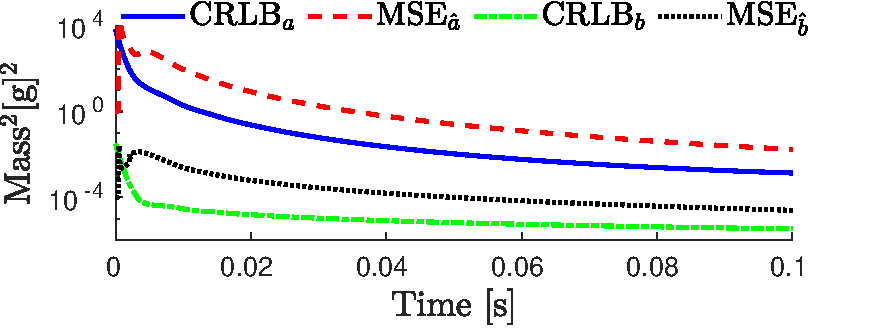
\includegraphics[width=0.69\columnwidth]{./ChapterRampInput/fig/Fig_5.pdf} 
\caption{ \label{fig:CRLB_MSE_ab_dd_40dB_MC_10000} When the SNR of the sensor response is 40 dB, the mean squared errors of the slope estimate $\widehat{a}$ and the intercept estimate $\widehat{b}$, obtained by the subspace method, are two orders of magnitude above the theoretical minimum variance given by the Cram\'er-Rao lower bound.}
\end{figure}


\begin{figure}[!htbp]
\centering
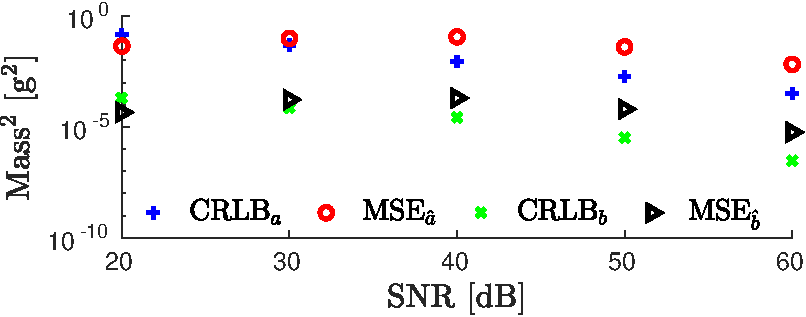
\includegraphics[width=0.69\columnwidth]{./ChapterRampInput/fig/Fig_6.pdf} 
\caption{ \label{fig:CRLB_MSE_SNR_ab_dd_MC_10000} The Cram\'er-Rao lower bounds of the estimates $\mathrm{CRLB}_a$ and $\mathrm{CRLB}_b$ determine the minimum uncertainty that can be achieved and increases with the measurement noise. 
The empirical mean squared errors $\mathrm{MSE}_{\hat{a}}$ and $\mathrm{MSE}_{\hat{b}}$ are near to the Cram\'er-Rao lower bounds within one order of magnitude for SNR smaller than 30 dB, and within two orders of magnitude for SNR between 40 dB and 60 dB. }
\end{figure}


\begin{table}[h!]
\centering
\caption{ The maximum values of the estimation mean squared errors observed when the subspace method processed the sensor transient responses caused by ramp excitations of masses 0.1, 0.3, 0.5, and 1.0 kg, that last 0.05, 0.1 and 0.5 s, with signal to noise ratios in the interval [20 dB, 60 dB] occur mainly at 40 dB and for lower SNR. There is an increment in the MSE values when the ramp excitation is faster.}
 
\begin{tabular}{l|l l l l} 
 \hline
 & Mass & \\ [0.5ex] 
 Time & 0.1 \ kg & 0.3 \ kg & 0.5 \ kg & 1.0 \ kg \\ 
 \hline
\multicolumn{1}{l|}{0.05 \ s} & \\
 \multicolumn{1}{r|}{\hspace{1mm} $\mathrm{MSE}_{\hat{a}} \ \mathrm{[g^2]}$} & $3.5\mathrm{x}10^{0}_{(@40 \ \mathrm{dB})}$ & $13.5\mathrm{x}10^{0}_{(@50 \ \mathrm{dB})}$ & $3.8\mathrm{x}10^{0}_{(@20 \ \mathrm{dB})}$ & $8.3\mathrm{x}10^{0}_{(@50 \ \mathrm{dB})}$ \\ 
\multicolumn{1}{r|}{\hspace{1mm} $\mathrm{MSE}_{\hat{b}} \ \mathrm{[g^2]}$} & $3.1\mathrm{x}10^{-3}_{(@40 \ \mathrm{dB})}$ & $1.1\mathrm{x}10^{-2}_{(@40 \ \mathrm{dB})}$ & $1.1\mathrm{x}10^{-2}_{(@40 \ \mathrm{dB})}$ & $1.9\mathrm{x}10^{-2}_{(@60 \ \mathrm{dB})}$ \\
\multicolumn{1}{l|}{0.1 \ s} & \\
 \multicolumn{1}{r|}{\hspace{1mm} $\mathrm{MSE}_{\hat{a}} \ \mathrm{[g^2]}$} & $3.1\mathrm{x}10^{-2}_{(@30 \ \mathrm{dB})}$ & $1.1\mathrm{x}10^{0}_{(@40 \ \mathrm{dB})}$ & $8.3\mathrm{x}10^{-1}_{(@60 \ \mathrm{dB})}$ & $1.3\mathrm{x}10^{0}_{(@50 \ \mathrm{dB})}$ \\
\multicolumn{1}{r|}{\hspace{1mm} $\mathrm{MSE}_{\hat{b}} \ \mathrm{[g^2]}$} & $6.0\mathrm{x}10^{-5}_{(@30 \ \mathrm{dB})}$ & $1.2\mathrm{x}10^{-1}_{(@50 \ \mathrm{dB})}$ & $2.1\mathrm{x}10^{-2}_{(@40 \ \mathrm{dB})}$ & $3.7\mathrm{x}10^{-2}_{(@40 \ \mathrm{dB})}$ \\
\multicolumn{1}{l|}{0.5 \ s} & \\
 \multicolumn{1}{r|}{\hspace{1mm} $\mathrm{MSE}_{\hat{a}} \ \mathrm{[g^2]}$} & $3.0\mathrm{x}10^{-2}_{(@20 \ \mathrm{dB})}$ & $3.0\mathrm{x}10^{-1}_{(@20 \ \mathrm{dB})}$ & $3.2\mathrm{x}10^{0}_{(@20 \ \mathrm{dB})}$ & $8.6\mathrm{x}10^{-2}_{(@20 \ \mathrm{dB})}$ \\
\multicolumn{1}{r|}{\hspace{1mm} $\mathrm{MSE}_{\hat{b}} \ \mathrm{[g^2]}$} & $3.1\mathrm{x}10^{-5}_{(@50 \ \mathrm{dB})}$ & $9.8\mathrm{x}10^{-4}_{(@40 \ \mathrm{dB})}$ & $2.0\mathrm{x}10^{-5}_{(@50 \ \mathrm{dB})}$ & $1.7\mathrm{x}10^{-5}_{(@20 \ \mathrm{dB})}$ \\ [0.5ex] % [\mathrm{samples}]
 \hline
\end{tabular}
\label{table:differentmasses}
\end{table}


A numerical sensitivity analysis of the subspace method was conducted by adding uncertainty to ramp input generation and looking into the estimation results. 
The uncertainty $\sigma_{\mathrm{s}}$ of the speed in which the ramp increases, and the uncertainties of the input parameters, represented by $\sigma_{a,b}$, were selected to be 0\%, 5\% and 10\% of their true values.
A Monte Carlo simulation with $10^4$ runs was performed for each SNR and the maximum values of the estimation uncertainty are shown in Table \ref{table:dd_sensitivity}. 
According to these results, the input parameters uncertainties $\sigma_{a,b}$ affect more the uncertainty of the estimation than the speed uncertainty $\sigma_{\mathrm{s}}$. 
The parameter that is more affected by the input parameters uncertainty is the intercept $\widehat{b}$, since the uncertainty of the slope $\widehat{a}$ is smaller.


\begin{table}[h!]
\centering
\caption{ A sensitivity analysis of the subspace method was conducted by adding uncertainty to the ramp input. The speed $\sigma_{\mathrm{s}}$, and the input parameters $\sigma_{\mathrm{s}}$ uncertainties are 0\%, 5\%, and 10\% of their true values. The table shows the maximum values of the estimation uncertainty. The speed uncertainty causes a smaller spread of the estimates than the input parameters uncertainty.}
 
\begin{tabular}{c| c c c} 
\hline  
$\sigma_{{a},{b}}$ & $\sigma_{\mathrm{s}}$: \ 0\% & 5\% & 10\% \\ [0.5ex] 
 \hline
 \multicolumn{1}{l|}{0\%} \\
 \multicolumn{1}{l|}{\hspace{2mm} $\widehat{a} \ \mathrm{[kg/s]}$} & $1.0 \pm 9.6 \%_{(@50 \ \mathrm{dB})}$ &  $1.0 \pm 8.2 \%_{(@20 \ \mathrm{dB})}$ & $1.0 \pm 8.2 \%_{(@50 \ \mathrm{dB})}$ \\ 
 \multicolumn{1}{l|}{\hspace{2mm} $\widehat{b} \ \mathrm{[g]}$} & $10.0 \pm 10.3 \%_{(@20 \ \mathrm{dB})}$ & $9.9 \pm 14.2 \%_{(@30 \ \mathrm{dB})}$ & $10.0 \pm 21.7 \%_{(@60 \ \mathrm{dB})}$ \\ 
 \multicolumn{1}{l|}{5\%} \\
 \multicolumn{1}{l|}{\hspace{2mm} $\widehat{a} \ \mathrm{[kg/s]}$} & $1.0 \pm 9.7 \%_{(@50 \ \mathrm{dB})}$ & $1.0 \pm 11.3 \%_{(@20 \ \mathrm{dB})}$ & $1.0 \pm 8.0 \%_{(@50 \ \mathrm{dB})}$ \\  
 \multicolumn{1}{l|}{\hspace{2mm} $\widehat{b} \ \mathrm{[g]}$} & $10.0 \pm 22.4 \%_{(@50 \ \mathrm{dB})}$ & $10.0 \pm 33.2 \%_{(@30 \ \mathrm{dB})}$ & $9.9 \pm 16.6 \%_{(@50 \ \mathrm{dB})}$ \\ 
\multicolumn{1}{l|}{10\%} \\
\multicolumn{1}{l|}{\hspace{2mm} $\widehat{a} \ \mathrm{[kg/s]}$} & $1.0 \pm 20.3 \%_{(@40 \ \mathrm{dB})}$ & $1.0 \pm 22.0 \%_{(@50 \ \mathrm{dB})}$ & $1.0 \pm 17.7 \%_{(@40 \ \mathrm{dB})}$ \\    
 \multicolumn{1}{l|}{\hspace{2mm} $\widehat{b} \ \mathrm{[g]}$} & $9.9 \pm 46.8 \%_{(@40 \ \mathrm{dB})}$ & $9.8 \pm 58.8 \%_{(@50 \ \mathrm{dB})}$ & $9.9 \pm 41.6 \%_{(@40 \ \mathrm{dB})}$ \\ [0.5ex] 
\hline
\end{tabular}
\label{table:dd_sensitivity}
\end{table}


\subsection{Results of the maximum-likelihood method}
\color{blue} 
The maximum-likelihood (ML) method estimates the affine input parameters from the sensor model transient response.
A total of 100 runs of the method were obtained, using different realizations of the measurement noise.
The measurement noise variance was set to have an SNR of 40 dB.
The ML method used the first 50 samples to initialize the optimization variables and updated the variables every $N_{\mathrm{s}} = 5$ samples.
Figure \ref{fig:rele_lo_40dB_s10} shows the average of the observed relative errors in the estimation of the parameters $\widehat{a}$, $\widehat{b}$, $\widehat{x}_{\mathrm{ini,1}}$, and $\widehat{x}_{\mathrm{ini,2}}$\color{black}.
The convergence of the ML estimates gives relative errors below 5 \% after three iterations.
The largest relative error observed is in the scale velocity $\widehat{x}_{\mathrm{ini,2}}$ estimate, which is more sensitive than the other optimization variables.


\begin{figure}[!htbp]
\centering
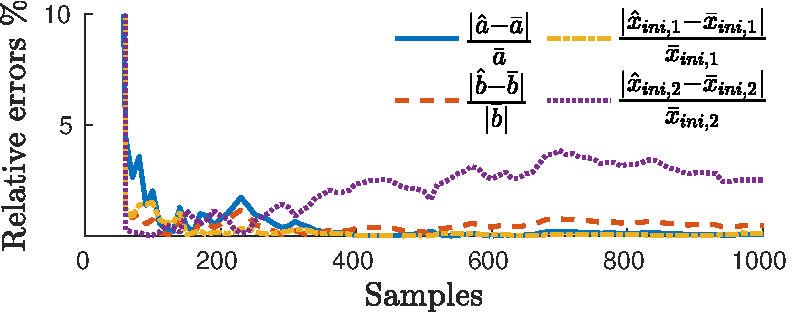
\includegraphics[width=0.69\columnwidth]{./ChapterRampInput/fig/Fig_7.pdf} 
\caption{ \label{fig:rele_lo_40dB_s10} The affine input parameters and the sensor's initial conditions are estimated with the ML method. After three iterations, \color{blue} the average of the relative error is smaller than 5 \% for each and every of the estimates. The estimate $\widehat{x}_{\mathrm{ini,2}}$ has the larger relative error near to 1 \%. \color{black} }
\end{figure}

The estimation covariance was computed using the analytic Jacobian and the Equation (\ref{eqn:covOpt}).
Figure \ref{fig:cov_lo_40dB_s1} shows \color{blue} the average \color{black} of the variances that were observed on the diagonal of the covariance matrix $\mathbf{J}$. 
We can see that the estimation variances decrease as more samples are processed.
Moreover, the estimation variances of $\widehat{a}$ and $\widehat{b}$ obtained with the ML method are lower than 
the corresponding estimation MSE errors obtained from a Monte Carlo simulation of the subspace method (see Figure \ref{fig:CRLB_MSE_SNR_ab_dd_MC_10000}).
  
\begin{figure}[!htbp]
\centering
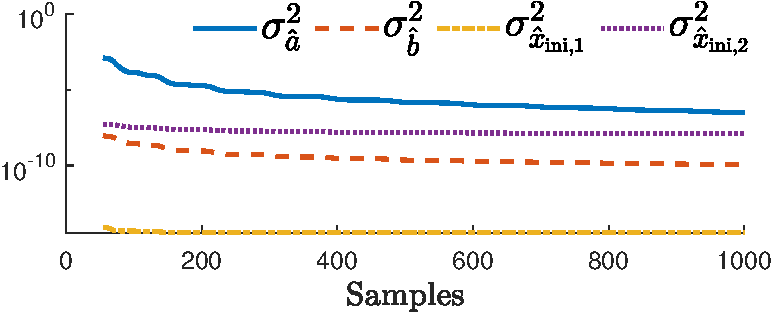
\includegraphics[width=0.69\columnwidth]{./ChapterRampInput/fig/Fig_8.pdf} 
\caption{ \label{fig:cov_lo_40dB_s1} The variances of the ML estimates are calculated using the information provided by the analytic Jacobian. \color{blue} The estimates $\widehat{x}_{\mathrm{ini,1}}$ and $\widehat{a}$ have the smaller and larger variances, respectively. \color{black}  }
\end{figure}

The ML method is computationally more expensive than the subspace method because the ML method simulates the response of a sensor model to optimize the input parameters and the sensor's initial conditions.

A typical run of the ML method takes 30 s to complete.
With this execution time, the ML estimation can only be performed offline.
Nevertheless, the ML method objectives are to give the best estimation possible and to serve as a reference to assess the results of the other methods.
An efficient implementation of the ML method to make it feasible for real-time implementation is not trivial and requires additional research that is considered a topic for future research.

A numerical sensitivity analysis of the ML method was conducted by adding uncertainty to the ramp input, and to the parameters of the time-varying model. 
The ramp input was perturbed with uncertainty of the speed in which the ramp increases $\sigma_{\mathrm{s}}$, and with uncertainty on the input parameters $\sigma_{a,b}$. 
The perturbation uncertainty of the model parameters $m$, $d$, and $k$ is represented by $\sigma_{m,d,k}$. 
The perturbation uncertainty was simulated by adding normally distributed random noise with standard deviation equal to 0\%, 5\% and 10\% of the corresponding true values of the perturbed parameters.
A Monte Carlo simulation with $10^3$ runs was conducted for each SNR in the SNR interval of interest, and in Table \ref{table:ml_sensitivity} are shown the maximum values of the observed estimation uncertainties. 
The results show that the speed uncertainty $\sigma_{\mathrm{s}}$ has a small impact on the estimation uncertainty.
On the contrary, the input parameters uncertainties $\sigma_{a,b}$, and the uncertainties of the model parameters $\sigma_{m,d,k}$ cause a large increment in the uncertainty of the estimation.

\begin{table}[h!]
\centering
\caption{ A sensitivity analysis of the ML method was conducted by adding uncertainty to ramp input, and to the model parameters. The perturbation uncertainty was selected with standard deviation of 0\%, 5\%, and 10\% of the parameters true values. The observed maximum estimation uncertainties are shown in the table. The speed uncertainty $\sigma_{\mathrm{s}}$ affects less the input estimation, but the uncertainties of the input parameters $\sigma_{a,b}$, and the model parameters $\sigma_{m,d,k}$ cause an increase of the estimation parameters spread around their mean values.}
 
\begin{tabular}{c| c c c} 
\hline  
$\sigma_{{a},{b}}$ & $\sigma_{\mathrm{s}}$: \ 0\% & 5\% & 10\% \\ [0.5ex] 
\hline
 \multicolumn{1}{l|}{0\%} \\
 \multicolumn{1}{l|}{\hspace{2mm} $\widehat{a} \ \mathrm{[kg/s]}$} & $1.0 \pm 0.7 \%_{(@20 \ \mathrm{dB})}$ &  $1.0 \pm 0.7 \%_{(@20 \ \mathrm{dB})}$ & $1.0 \pm 0.4 \%_{(@30 \ \mathrm{dB})}$ \\ 
 \multicolumn{1}{l|}{\hspace{2mm} $\widehat{b} \ \mathrm{[g]}$} & $10.0 \pm 1.1 \%_{(@20 \ \mathrm{dB})}$ & $10.0 \pm 1.1 \%_{(@20 \ \mathrm{dB})}$ & $10.0 \pm 0.5 \%_{(@30 \ \mathrm{dB})}$ \\ 
 \multicolumn{1}{l|}{\hspace{2mm} $\widehat{x}_{\mathrm{ini,1}} \ \mathrm{[g]}$} & $0.1 \pm 0.6 \%_{(@40 \ \mathrm{dB})}$ & $0.1 \pm 0.6 \%_{(@20 \ \mathrm{dB})}$ & $0.1 \pm 0.2 \%_{(@30 \ \mathrm{dB})}$ \\
 \multicolumn{1}{l|}{\hspace{2mm} $\widehat{x}_{\mathrm{ini,2}} \ \mathrm{[g/s]}$} & $0.1 \pm 122 \%_{(@40 \ \mathrm{dB})}$ & $0.1 \pm 130 \%_{(@40 \ \mathrm{dB})}$ & $0.1 \pm 38 \%_{(@50 \ \mathrm{dB})}$ \\
 \multicolumn{1}{l|}{5\%} \\
 \multicolumn{1}{l|}{\hspace{2mm} $\widehat{a} \ \mathrm{[kg/s]}$} & $1.0 \pm 9.0 \%_{(@50 \ \mathrm{dB})}$ & $1.0 \pm 5.2 \%_{(@40 \ \mathrm{dB})}$ & $1.0 \pm 5.6 \%_{(@40 \ \mathrm{dB})}$ \\  
 \multicolumn{1}{l|}{\hspace{2mm} $\widehat{b} \ \mathrm{[g]}$} & $9.9 \pm 25.4 \%_{(@50 \ \mathrm{dB})}$ & $10.0 \pm 5.2 \%_{(@20 \ \mathrm{dB})}$ & $10.0 \pm 4.7 \%_{(@40 \ \mathrm{dB})}$ \\ 
\multicolumn{1}{l|}{\hspace{2mm} $\widehat{x}_{\mathrm{ini,1}} \ \mathrm{[g]}$} & $0.1 \pm 0.6 \%_{(@20 \ \mathrm{dB})}$ & $0.1 \pm 0.6 \%_{(@20 \ \mathrm{dB})}$ & $0.1 \pm 6.2 \%_{(@30 \ \mathrm{dB})}$ \\
 \multicolumn{1}{l|}{\hspace{2mm} $\widehat{x}_{\mathrm{ini,2}} \ \mathrm{[g/s]}$} & $40.1 \pm 116 \%_{(@40 \ \mathrm{dB})}$ & $0.1 \pm 128 \%_{(@40 \ \mathrm{dB})}$ & $0.1 \pm 115 \%_{(@40 \ \mathrm{dB})}$ \\
 \multicolumn{1}{l|}{10\%} \\
 \multicolumn{1}{l|}{\hspace{2mm} $\widehat{a} \ \mathrm{[kg/s]}$} & $1.0 \pm 10.4 \%_{(@30 \ \mathrm{dB})}$ & $1.0 \pm 10.3 \%_{(@20 \ \mathrm{dB})}$ & $1.0 \pm 10.3 \%_{(@20 \ \mathrm{dB})}$ \\ 
 \multicolumn{1}{l|}{\hspace{2mm} $\widehat{b} \ \mathrm{[g]}$} & $9.9 \pm 10.5 \%_{(@20 \ \mathrm{dB})}$ & $9.9 \pm 10.4 \%_{(@20 \ \mathrm{dB})}$ & $10.0 \pm 10.5 \%_{(@20 \ \mathrm{dB})}$ \\ 
\multicolumn{1}{l|}{\hspace{2mm} $\widehat{x}_{\mathrm{ini,1}} \ \mathrm{[g]}$} & $0.1 \pm 0.6 \%_{(@20 \ \mathrm{dB})}$ & $0.1 \pm 0.6 \%_{(@20 \ \mathrm{dB})}$ & $0.1 \pm 0.6 \%_{(@20 \ \mathrm{dB})}$ \\
 \multicolumn{1}{l|}{\hspace{2mm} $\widehat{x}_{\mathrm{ini,2}} \ \mathrm{[g/s]}$} & $0.1 \pm 108 \%_{(@50 \ \mathrm{dB})}$ & $0.1 \pm 110 \%_{(@40 \ \mathrm{dB})}$ & $0.1 \pm 137 \%_{(@50 \ \mathrm{dB})}$ \\ 
 \hline
 $\sigma_{{m},{d},{k}}$ & $\sigma_{\mathrm{s}}$: \ 0\% & 5\% & 10\% \\
 \hline
 \multicolumn{1}{l|}{0\%} \\
 \multicolumn{1}{l|}{\hspace{2mm} $\widehat{a} \ \mathrm{[kg/s]}$} & $1.0 \pm 0.7 \%_{(@20 \ \mathrm{dB})}$ &  $1.0 \pm 0.7 \%_{(@20 \ \mathrm{dB})}$ & $1.0 \pm 0.3 \%_{(@30 \ \mathrm{dB})}$ \\ 
 \multicolumn{1}{l|}{\hspace{2mm} $\widehat{b} \ \mathrm{[g]}$} & $10.0 \pm 1.1 \%_{(@20 \ \mathrm{dB})}$ & $10.0 \pm 1.1 \%_{(@20 \ \mathrm{dB})}$ & $10.0 \pm 0.4 \%_{(@30 \ \mathrm{dB})}$ \\ 
 \multicolumn{1}{l|}{\hspace{2mm} $\widehat{x}_{\mathrm{ini,1}} \ \mathrm{[g]}$} & $0.1 \pm 0.6 \%_{(@40 \ \mathrm{dB})}$ & $0.1 \pm 0.2 \%_{(@30 \ \mathrm{dB})}$ & $0.1 \pm 0.2 \%_{(@30 \ \mathrm{dB})}$ \\
 \multicolumn{1}{l|}{\hspace{2mm} $\widehat{x}_{\mathrm{ini,2}} \ \mathrm{[g/s]}$} & $0.1 \pm 122 \%_{(@40 \ \mathrm{dB})}$ & $0.1 \pm 130 \%_{(@40 \ \mathrm{dB})}$ & $0.1 \pm 38 \%_{(@50 \ \mathrm{dB})}$ \\
 \multicolumn{1}{l|}{5\%} \\
 \multicolumn{1}{l|}{\hspace{2mm} $\widehat{a} \ \mathrm{[kg/s]}$} & $1.0 \pm 15.3 \%_{(@20 \ \mathrm{dB})}$ & $1.0 \pm 0.7 \%_{(@20 \ \mathrm{dB})}$ & $1.0 \pm 21.5 \%_{(@20 \ \mathrm{dB})}$ \\  
 \multicolumn{1}{l|}{\hspace{2mm} $\widehat{b} \ \mathrm{[g]}$} & $10.3 \pm 79.4 \%_{(@20 \ \mathrm{dB})}$ & $10.0 \pm 1.2 \%_{(@20 \ \mathrm{dB})}$ & $9.9 \pm 19.0 \%_{(@20 \ \mathrm{dB})}$ \\ 
\multicolumn{1}{l|}{\hspace{2mm} $\widehat{x}_{\mathrm{ini,1}} \ \mathrm{[g]}$} & $0.1 \pm 0.2 \%_{(@30 \ \mathrm{dB})}$ & $0.1 \pm 0.6 \%_{(@20 \ \mathrm{dB})}$ & $0.1 \pm 0.2 \%_{(@20 \ \mathrm{dB})}$ \\
 \multicolumn{1}{l|}{\hspace{2mm} $\widehat{x}_{\mathrm{ini,2}} \ \mathrm{[g/s]}$} & $0.1 \pm 113 \%_{(@40 \ \mathrm{dB})}$ & $0.1 \pm 119 \%_{(@40 \ \mathrm{dB})}$ & $0.1 \pm 323 \%_{(@30 \ \mathrm{dB})}$ \\
 \multicolumn{1}{l|}{10\%} \\
 \multicolumn{1}{l|}{\hspace{2mm} $\widehat{a} \ \mathrm{[kg/s]}$} & $1.0 \pm 22 \%_{(@30 \ \mathrm{dB})}$ & $1.0 \pm 16 \%_{(@30 \ \mathrm{dB})}$ & $1.0 \pm 28 \%_{(@50 \ \mathrm{dB})}$ \\ 
 \multicolumn{1}{l|}{\hspace{2mm} $\widehat{b} \ \mathrm{[g]}$} & $0.1 \pm 26 \%_{(@30 \ \mathrm{dB})}$ & $9.9 \pm 14.8 \%_{(@30 \ \mathrm{dB})}$ & $10.4 \pm 93 \%_{(@50 \ \mathrm{dB})}$ \\ 
\multicolumn{1}{l|}{\hspace{2mm} $\widehat{x}_{\mathrm{ini,1}} \ \mathrm{[g]}$} & $0.1 \pm 0.6 \%_{(@20 \ \mathrm{dB})}$ & $0.1 \pm 0.6 \%_{(@20 \ \mathrm{dB})}$ & $0.1 \pm 0.6 \%_{(@20 \ \mathrm{dB})}$ \\
 \multicolumn{1}{l|}{\hspace{2mm} $\widehat{x}_{\mathrm{ini,2}} \ \mathrm{[g/s]}$} & $0.1 \pm 121 \%_{(@40 \ \mathrm{dB})}$ & $0.1 \pm 136 \%_{(@40 \ \mathrm{dB})}$ & $0.1 \pm 111 \%_{(@40 \ \mathrm{dB})}$ \\  [0.5ex] 
\hline
\end{tabular}

\label{table:ml_sensitivity}
\end{table}




\subsection{Results of the time-varying filter}

We fixed the frequency lower value $f_l=0.01$ Hz and the base $\beta = 0.01$. 
The upper value $f_u$ and the decay rate $\alpha$ were found using optimization (\ref{eqn:tv_optim}). 
We chose the values $\mu_{\mathrm{spec}}=0.5$ and $\sigma_{\mathrm{spec}}=0.24$ as they are specified in the OIML recommendation defined in \citet{OIML_R51_1} for a mass of 100 g measured in a conveyor belt.
The optimized values of the frequency upper value and the decay rate, using a dataset of 100 transient responses, were $f_u = 26.94$ Hz and $\alpha = 5.71$.

Figure \ref{fig:rele_tv_40dB_s1} shows the relative errors of the estimates $\widehat{a}$ and $\widehat{b}$ computed with the TV filter after processing the sensor transient response.
The relative error of the slope estimate is below 5 \% after 300 samples but the relative error of the intercept estimate is near 10 \%.
The convergence rate of the estimate $\widehat{a}$ was similar to that of the subspace method.

\begin{figure}[!htbp]
\centering
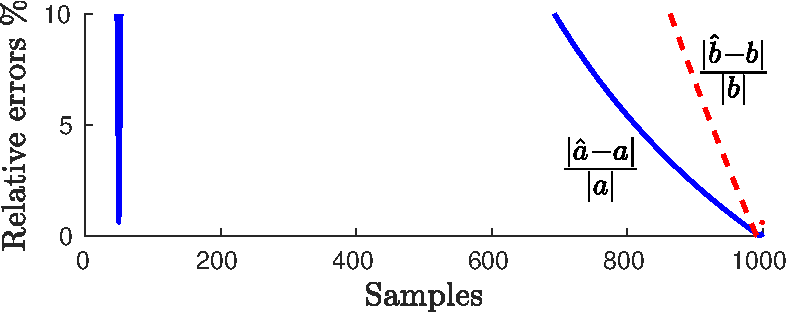
\includegraphics[width=0.69\columnwidth]{./ChapterRampInput/fig/Fig_9.pdf} 
\caption{ \label{fig:rele_tv_40dB_s1} The relative errors of the time-varying filter estimation converge slower than with the subspace method. 
The relative errors of $\widehat{a}$ and $\widehat{b}$ are smaller than 5 \% only after 800 and 950 samples, respectively.
With the subspace method the relative errors are below 5 \% after 400 and 500 samples. }
\end{figure}



\subsection{Discussion of the observed results}

The subspace method obtains an estimation of the affine input parameters with a recursive least-squares solution of a structured errors-in-variables problem.
Updating the parameter estimates without matrix inversion simplifies the method implementation on digital signal processors of low cost.
The price we pay by computing the least-squares solution of an errors-in-variables problem is an increase in the bias of the estimates.
Nevertheless, the empirical mean squared errors of the estimates are at most two orders of magnitude larger than the Cram\'er-Rao lower bound, meaning that the estimation uncertainty is low, even when the SNR is lower than 40 dB.


The proposed subspace method is a general method that can be used in different applications, with realistic signal-to-noise ratios. 
It is suitable not only for mass measurements.
The weighing example shows that the subspace method can be used even when the measurement system is linear time-varying.

It was shown that the time-varying (TV) compensation filter can be modified to estimate the mass only from the increasing section of the saturated ramp, without the need of processing the saturation part.
The modified TV filter can be implemented in real-time as the subspace method after a previous off-line coefficients optimization stage with sensor measured data.
Nevertheless, the estimation results of the subspace method are better than the TV filter since they are twice as fast and one order of magnitude more acurate.

The subspace method can estimate the affine input parameters from the sensor response using few parameters, the sensor order $n$, the sensor static gain ${G}$, and the RLS forgetting factor $\omega$.
The subspace method does not necessarily requires optimization of $\omega$ using a dataset of measured sensor responses.
It is required to tune $\omega$ online during the calibration of the system and later $\omega$ remains fixed during the measurements.

The results of the sensitivity analysis show how the uncertainty of the subspace method estimates is affected when the ramp input is subject to perturbation.
The impact on the uncertainty on the slope $\widehat{a}$ and the intercept $\widehat{b}$ parameters is different.
The ramp speed uncertainty $\sigma_{\mathrm{s}}$ is added to the uncertainty of the parameter $\widehat{b}$, but does not contribute to the uncertainty of the parameter $\widehat{a}$.
On the other hand, the ramp parameters uncertainty ramp speed uncertainty $\sigma_{a,b}$ is added to the uncertainty of the estimates of both parameters $\widehat{a}$ and $\widehat{b}$.
This is not surprising since the estimation parameters are linked to the ramp input parameters.

The maximum-likelihood (ML) method is an approach that requires larger computational resources.
This is an iterative method and in each iteration computes a simulation of a dynamic system followed by the evaluation of the residual error Jacobian matrix.
The advantage of the ML method is that we can estimate simultaneously sensor parameters and the initial conditions of the sensor.
In the weighing case presented as an illustrative example it was not possible to incorporate other parameters of the sensor because they are not identifiable.
According to the estimation relative errors, that are lower than 0.01 after 100 samples, from there on the ML method estimates are near to the true values and we may not require to run the method along all the measurement period.
With only the first 100 samples we have an accurate parameter estimation and variance assessment.

However, the main drawback of the ML method that prevents online implementations is the required computational power to iteratively simulate the response of a sensor model.
It takes an average of 30 s to complete an estimation with the ML method, and this time is too large for fast changing inputs.
The development of an efficient ML method, suitable for real-time implementation, is not straightforward, and is proposed for future research.

The results of the sensitivity analysis of the ML method show that the uncertainty of the ramp input speed $\sigma_{\mathrm{s}}$ does not have an impact on the estimation uncertainty.
Similar to the subspace case, the uncertainty of the ramp input parameters $\sigma_{a,b}$ is additive to the uncertainty of the estimated parameters $\widehat{a}$ and $\widehat{b}$, but does not contribute to the uncertainty of the first element of the initial conditions.
On the other hand, the estimation uncertainty is affected by the perturbation on the model parameters $\sigma_{m,d,k}$.
It is observed that the uncertainty of the estimated parameters $\widehat{a}$ and $\widehat{b}$ increases two and three times the uncertainty of the model parameters.
This implies that we need to have an accurate model of the dynamic system to have a small uncertainty on the estimated input parameters.
Unfortunately, the uncertainty of the second element of the inital conditions is always very high and this is not because of the perturbation of the ramp speed or the model parameters. 
This issue requires more investigation to see if it is due the identifiability of the parameter in the particular example we have.


\section{Conclusions}

An adaptive subspace method was proposed for estimating affine input parameters given the measurement of the caused sensor transient response. 
The subspace estimation method is a recursive method that allows online implementation.
This method tracks the input of a system, using exponential forgetting, to process the system response.
The subspace method is model-free and estimates directly the input parameters without identifying a sensor model.
Therefore, it can be applied to the measurement of different physical magnitudes.
In the specific weighing example described in the manuscript, the input is an affine function.
The method is also applicable when the sensor is time-varying.
The subspace method is computationally cheap, simple and suitable for implementation on digital signal processor of low computational power. 

A maximum-likelihood estimator based on local optimization was designed to obtain a comparative reference for the other methods.
The maximum-likelihood method estimates the affine input parameters and also model parameters and the sensor's initial conditions.
This method simulates, in a receding horizon scheme, the response of a sensor model to estimate the input and minimizes the sum of the squares of the residual between the measured and the estimated responses.
The main drawback of the maximum-likelihood method is its computational cost and efficient implementation of the method is left for future work.

A linear time-invariant weighing system is used as a test example for the estimation methods.
The weighing system becomes time-varying when an affine input excites the system.
The estimation methods are compared in a simulation study where the time-varying sensor response is perturbed by measurement noise, that is assumed to be white, of zero mean, and with known finite variance.
The subspace method results are also compared to those of an existing digital time-varying filter.
The coefficients of the time-varying filter require offline optimization.
The estimation results obtained with the subspace method converges two times faster and is one order of magnitude smaller than those obtained with the time-varying filter.
The empirical mean squared errors of the subspace method estimation is two orders of magnitude larger than the theoretical minimum given by the Cram\'er-Rao Lower bound.

Future work of this research is the practical implementation of the subspace method for real-time measurements.

%\newpage
